\label{sec:planning}

In this section, we will provide a detailed introduction to the high-level planner, which constitutes the upper layer of the framework. It processes input from point clouds and robot proprioception, and outputs the manipulation trajectory parameters for the end-effector.

\subsubsection{Framework}
Our planner $\pi_{p}$ utilizes DP3~\cite{ze2024DP3} as the backbone, which is a diffusion-based 3D visuomotor policy that can efficiently process 3D data and learn the manipulation trajectory of end-effector from expert demonstrations.

\paragraph{Input}
 We utilize proprioceptive data of the robot state $s_{t}$ and visual point cloud data ${}^{w}\mathbf{P} \in  \mathbb{R}^{n\times 3}$ as inputs. The visual data is captured by a depth camera mounted behind the robot and on its head, which is then transformed into point clouds in the world frame. During the manipulation process, we randomly sample $n=768$ points to form the point clouds.
 
\paragraph{Output}
Our planner generates the parameters ${}^{w}p$ for the manipulation trajectory of the end-effector, represented in the world frame. These parameters can be used to calculate the target point, target orientation, and the manipulator flag $f$ at each moment of the manipulation process. This information is then fed into the subsequent low-level controller.

\subsubsection{Expert Demonstration Collection}

We represent the expert demonstration data as $\begin{aligned}\mathcal{D}=\{\xi_0,\xi_1\ldots\xi_n\}\end{aligned}$, where each trajectory $\xi_i=\{({}^{w}\mathbf{P}_i,s_i,{}^{w}p_i)\}$ is a sequence of point cloud observations ${}^{w}\mathbf{P}$, the robot proprioceptive state $s$, and trajectory parameters ${}^{w}p$.

As illustrated in Fig.~\ref{fig:expert_demo_line}, we designed expert trajectory parameters ${}^{o}p$ for different objects and tasks. To enable the robot to learn to manipulate objects placed in different poses, we randomized the positions and yaw axis angles of the objects. The expert trajectory parameters are represented in the object frame, allowing them to accurately follow the object. During the collection of expert demonstrations, the object frame is transformed to the world frame based on the object's pose.

We gather expert data by having robots follow expertly designed trajectories, utilizing large-scale parallel simulations in IsaacGym~\cite{makoviychuk2021isaac}. This method enables the rapid collection of a significant volume of data.

The collection time does not increase with the volume of data; it primarily depends on the size of the Video Random Access Memory (VRAM). In this paper, we collect 200 timesteps of expert demonstration data for each task, with 100 trajectories collected per task, taking approximately three minutes.

Despite the collection of expert data in simulations, our method achieves sim-to-real seamless deployment in actual environments, thanks to the point clouds post-process and carefully designed hierarchical structure.

\begin{figure}[t]
    \centering
    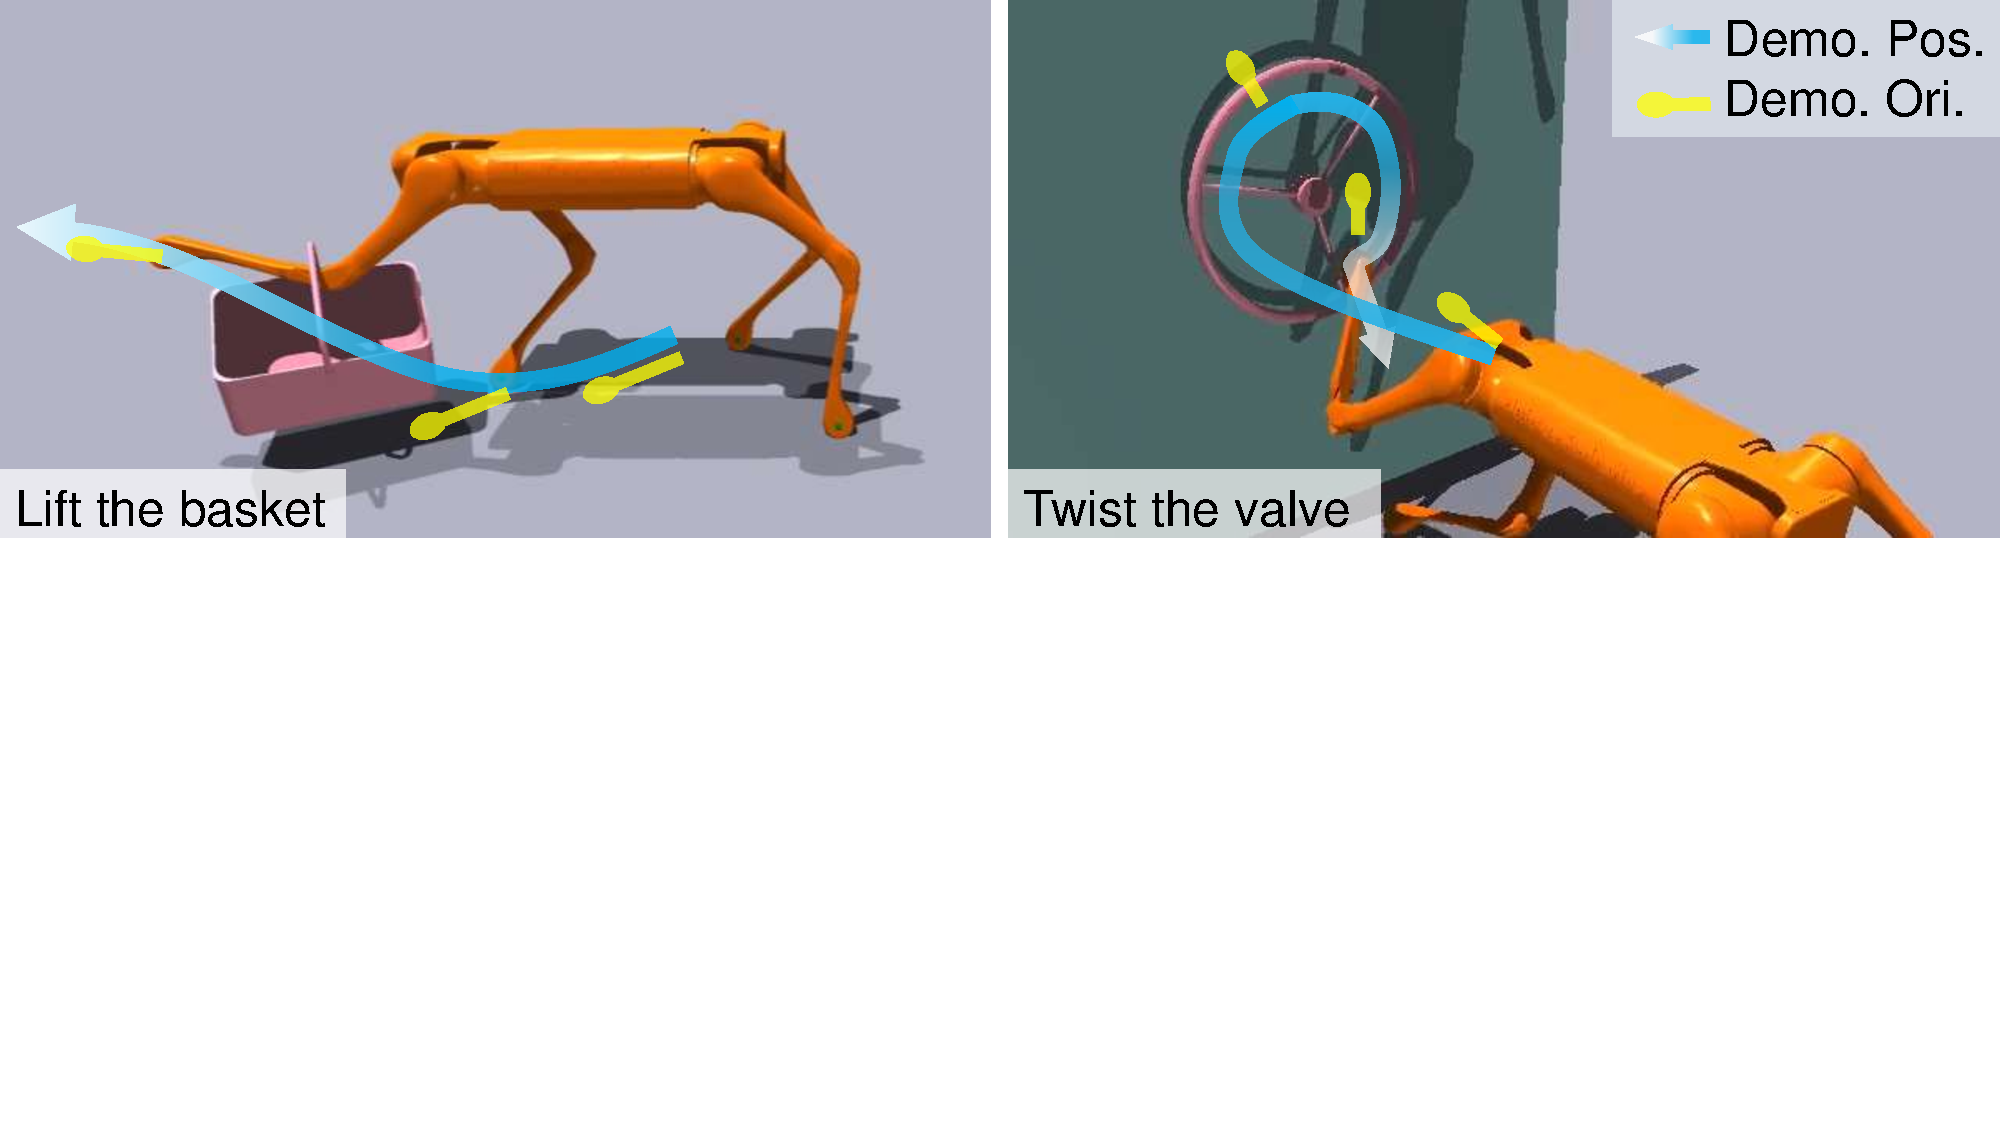
\includegraphics[width=\linewidth, trim={0 92mm 0 0}, clip]{figures/tasks_line/task_lines.pdf}
    \caption{Expert Demonstration. For different objects and tasks, we designed expert trajectory parameters and randomized the poses of the objects. The blue gradient curve represents the demonstration trajectory, and the yellow arrow indicate the demonstration orientation.}
    \label{fig:expert_demo_line}
    \vspace{-.2in}
\end{figure}

